\documentclass[8pt,a4paper,landscape]{extarticle}
% -- Layout ----
\usepackage[top=0.6cm, bottom=0.6cm, left=0.5cm, right=0.5cm, landscape]{geometry}

% -- Titles ----
\usepackage[
  tiny,                     % text size title
  compact                   % reduce vertical space before/after title
]{titlesec}
% \titlespacing*
\titleformat{\section}{\normalfont\small\bfseries}{\thesection}{0em}{} % Remove space before and after section titles
\titleformat{\subsection}{\normalfont\small\bfseries}{\thesubsection}{0em}{} % Remove space before and after subsection titles
\titlespacing*{\section}{0pt}{0pt}{0pt} % Remove space before/after section titles
\titlespacing*{\subsection}{0pt}{0pt}{0pt} % Remove space before/after subsec titles

% -- Colors ----
\usepackage[dvipsnames]{xcolor}
\definecolor{dmm}{RGB}{192,192,192} % Define a custom dimmed text color
\definecolor{cmt}{RGB}{61,123,123}

% -- Math ------
\usepackage{mathtools}
\usepackage{amssymb}
\usepackage{turnstile}%better vdash

% -- Lists -----
\usepackage[inline]{enumitem}
\setlist{noitemsep}% Remove vspace between items
% Set vspace before and after  list environments as well as the left margin
\setlist[itemize,1]{leftmargin=.6em,labelindent=0pt,labelsep=2pt,
  topsep=1pt,partopsep=1pt}
\setlist[enumerate,1]{leftmargin=1em,labelindent=0pt,labelsep=2pt,
  topsep=1pt,partopsep=1pt}
\setlist[itemize,2]{leftmargin=.3em,labelindent=1pt,topsep=1pt,partopsep=1pt}
\setlist[enumerate,2]{leftmargin=0.2em,labelindent=1pt,topsep=1pt,partopsep=1pt}
\setlist[description]{labelwidth=\linewidth,font=\small\bfseries,leftmargin=1em,topsep=1pt,partopsep=1pt}
% -- Code listing ---
\usepackage{listings}
\lstset{
  aboveskip=3pt,
  belowskip=3pt,
  basicstyle=\small\ttfamily,
  breaklines=true,
  % commentstyle=\upshape\ttfamily,
  captionpos=b,
  commentstyle=\color{cmt},
  frame=single,
  keepspaces=false,
  keywordstyle=\bfseries,
  showspaces=false,
  showstringspaces=false,
  showtabs=false,
  tabsize=2,
}

% Parse Trees
\usepackage{tikz}
\usetikzlibrary{ arrows, automata, bbox, calc, positioning,  decorations.pathmorphing, decorations.pathreplacing, decorations.shapes, }
\tikzset{
% ->, % makes the edges directed
>=stealth', % makes the arrow heads bold
node distance=1cm, % specifies minimum distance between two nodes
% small/.style={},
every state/.style={thick}, % sets the properties for each ’state’ node
every node/.style={inner sep=1pt},
initial text=start, % sets the text that appears on the start arrow
}

% Place a figure env right here via [H] option
\usepackage{float}

% Side by side figure
\usepackage{subcaption}
% \usepackage{caption}
% \captionsetup{belowskip=0pt, aboveskip=0pt}


% -- Multi-Col layout --
\usepackage{multicol}

% No indentation
\setlength\parindent{0pt}
\setlength\abovedisplayskip{-5pt}
\setlength\belowdisplayskip{-5pt}
\setlength\abovedisplayshortskip{-4pt}
\setlength\belowdisplayshortskip{-4pt}
\newcommand{\gor}{\;|\;}
\newcommand{\num}{\texttt{\#}~}
\renewcommand{\arraystretch}{1.2}


\begin{document}
% Suppress page number for all pages
\pagestyle{empty}

% Notes begin
\begin{multicols*}{3}
  % \section*{Jargon}
\begin{description}

\item[synchronous iteration] several procs start together at the beginning of each iteration and the next iteration must wait for all procs to finish current iteration

\item[SPMD] all procs execute the same program (Single Program, SP) in parallel (except for a small number of procs such as root), but each has its own set of data (Multiple Data). In src code, usually a proc ID is used to uniquely label a proc

\item[Motivation for parallelism]
  \begin{enumerate*}
  \item speed/performance (1h vs 1w)
  \item tackle larger-scale problems
  \item keep power consumption and heat dissipation under control
  \item more $\cdots$
  \end{enumerate*}

\item[peak flops/sec] $ = \# \text{cores} \times [\# \text{sockets}] \times \# \text{flops} \times \text{freq}$

\item[speedup (hard due to overheads)]
  \begin{enumerate*}
  \item idling (unbalanced load, sync, serial parts, etc)
  \item splitting computation into tasks
  \item communications among processes
  \end{enumerate*}

\item[speedup (fixed problem size) and efficiency] $S_p = \frac{T_{seq}}{T_{par}} (\geq 1)\qquad E_p = \frac{S_{p}}{p} (0 < E_p \leq 1)$

% \item[efficiency] $E_p = \frac{S_{p}}{p} (0 < E_p \leq 1)$

\item[embarrassingly (easy) parallel] aka. perfectly parallel, delightfully parallel or pleasingly parallel, where problem can be easily divided into independent parts and solved without communication

\item[strong scalability] fixed problem size + increasing $\# p \rightarrow$ perf $\downarrow$

\item[weak scalability] increasing $\# p$ and problem size $\rightarrow$ perf $\downarrow$

\item[communication latency] time taken to communicate a msg between 2 procs in a network

\item[minimal routing] takes 1 of shortest paths (XY-routing; E-cube)

\item[non-minimal routing] route the message along a longer path to avoid network congestion

\item[deterministic] routing determines a unique path \emph{solely} based on src and dest nodes

\item[adaptive] routing uses info on network state to determine message path

\item[walltime] the actual time taken from the start of a computer program to the end. aka. elapsed real time, real time, wall-clock time
\item[flops] floating-point operations (add, subtract, multiply, divide) per second
\item[ceil] ceil(n,p) = $(n + p - 1) / p$ especially when $n$ isn't evenly divisible by $p$

\item[synchronous] 2 procs A, B. A will only start sending when B explicitly signals it is ready to receive.  If not, A just waits (also blocks).  In such mode, two procs communicate with each other directly.

\item[asynchronous] All concurrent tasks execute asynchronously; possible to implement any parallel algorithm.  However, it is hard to reason about the program because of non-deterministic behavior due to race conditions.

\item[loosely synchronous] a good compromise between aysnc and sync.  Tasks and subtasks synchronize to perform interactions (easy to debug), while between interactions, tasks execute completely asynchronously.

\item[blocking, non-buffered] A sends and B recvs, no system buffer available.  A must hold the data (A being idle and blocking) until B is ready to receive.

\item[blocking, buffered] data/message can be copied into a system-controlled block of memory (buffer on A or B or both) so A can continue to execute.  When B is ready, it copies the buffered data into its own appropriate memory.  A \textbf{common} implementation is to buffer relatively small messages and switch to non-buffered mode for large messages (blocking too).  In general, better to write programs with bounded buffer requirements.  This blocking time is only the period of copying data into/from buffer.
\item[non-blocking] generally accompanied by a \texttt{check-status} operation.  Upon return from non-blocking send/recv, the proc is free to perform any computation that doesn't require communication.  Later the proc \textbf{checks} if non-blocking op has completed and wait for its completion if needed.
\item[communication domain] a set of processes allowed to communicate with each other.  Info about this domain is stored in vars of type \texttt{MPI\_Comm} aka \textbf{communicators} (used as arg to all message transfer MPI routines and they uniquely identify procs). One proc can belong to many different (possibly overlapping) communication domains.  \texttt{MPI\_COMM\_WORLD} includes all procs in parallel execution as they all may need to talk to each other.

\item[one-to-all broadcast] a single process sends \textbf{identical} data to all other processes or to a subset of them.  Initially, only the source process has the data of size $m$ that needs to be broadcast.  At the termination of the procedure, there are $p$ copies of the initial data --- one belonging to each process.

\item[all-to-one reduction] each of the p participating processes starts with a buffer $M$ containing $m$ words.  The data from all processes are combined through an associative operator and accumulated at a single destination process into one buffer of size $m$.  Reduction can be used to find the sum, product, maximum, or minimum of sets of numbers

\item[latency] At the logical level, a memory system (of multiple levels of caches) takes in a request for a memory word and returns a block of data of size $b$ containing the requested word after $l$ nanoseconds, referred to as the \textbf{latency} of the memory.  As an analogy, if water comes out of the end of a fire hose 2 seconds after a hydrant is turned on, then the latency of the system is 2 seconds.


\item[bandwidth] The rate at which data can be pumped from the memory to the processor determines the bandwidth of the memory system.  How much data (per unit time) gets transferred from memory to processor.


\item[hit ration] The fraction of data references satisfied by the cache is called the cache hit ratio of the computation on the system.   The effective computation rate of many applications is bounded \emph{not} by the processing rate of the CPU, but by the rate at which data can be pumped into the CPU.  Such computations are referred to as being \textbf{memory bound}.


\item[temporal locality] If at one point a particular mem location is ref-ed, then it's likely that the same location will be ref-ed again soon

\item[spatial locality] Data that is accessed or referenced spatially close to each other (\texttt{a[i-1],a[i],a[i+1]}) is likely to be accessed again in the near future

\item[recursive decomposition] a method for inducing concurrency in problems that can be solved using the divide-and-conquer strategy.  A problem is solved by first dividing it into a set of independent subproblems. Each subproblem is solved by recursively applying a similar division into smaller subproblems followed by a combination of their results. (quicksort)


\item[data decomposition] a powerful/commonly used method for deriving concurrency in algorithms that operate on large data structures.  The decomposition of computations is done in two steps.  First, the data on which the computations are performed is partitioned; second, this data partitioning is used to induce a partitioning of the computations into tasks. The operations these tasks perform on different data partitions are usually similar or are chosen from a small set of operations (LU factorization).


\item[partitioning output data] In many computations, each element of the output can be computed naturally independently of others as a function of the input. In such computations, a partitioning of the output data automatically induces a decomposition of the problems into tasks, where each task is assigned the work of computing a portion of the output. (matrix-multiplication)


\item[partioning input data] When impossible to split output data, it is possible to partition the input data, and then use this partitioning to induce concurrency. A task is created for each partition of the input data and this task performs as much computation as possible using these local data. Note that the solutions to tasks induced by input partitions may not directly solve the original problem. In such cases, a follow-up computation is needed to combine the results. (sum of n elements)

\item[exploratory decomposition] is used to decompose problems whose underlying computations correspond to a search of a space for solutions. In exploratory decomposition, we partition the search space into smaller parts, and search each one of these parts concurrently, until the desired solutions are found. For an example of exploratory decomposition, consider the 15-puzzle problem.


\item[speculative decomposition] used when a program may take one of many possible computationally significant branches depending on the output of other computations that precede it. In this situation, while one task is performing the computation whose output is used in deciding the next computation, other tasks can concurrently start the computations of the next stage. The speedup due to speculative decomposition can add up if there are multiple speculative stages. (discrete event simulation)


\item[stream parallelism] simultaneous execution of different programs on a data stream


\item[startup time $t_s$] The startup time is the time required to handle a message at the sending and receiving nodes: the time to prepare the message (adding header, trailer, and error correction information), the time to execute the routing algorithm, and the time to establish an interface between the local node and the router. This delay is incurred only once for a single message transfer

\item[per-hop time $t_h$ (aka. node latency)] After a message leaves a node, it takes a finite amount of time to reach the next node in its path. The time taken by the header of a message to travel between two directly-connected nodes in the network is called the per-hop time.


\item[per-word transfer time $t_w$] If the channel bandwidth is $r$ words/s, then each word takes time $tw = 1/r$ to traverse the link. This time is called the per-word transfer time. This time includes network as well as buffering overheads.




\end{description}

  %\pagebreak
% \section*{Amdahl's law (strong scaling law, \textbf{L5P5})}
\begin{equation}
  \label{eq:amdahl}
  S_p = \frac{T_{seq}}{T_{par}} = \frac{p}{pf + (1-f)} = \frac{1}{f + \frac{1-f}{p}}
\end{equation}
where $f$ is the serial portion that cannot be parallelized
\begin{tabular}{c|c}
  \hline
  \multicolumn{2}{l}{$S \rightarrow ? $ if run on 1000 CPU and 10\% ($f$) remains sequential} \\
  \hline
  $S_{ser} \quad p = 1$ & $S_{par} \quad p = 1000$  \\
  \hline
  2GFLOP/s  & $S_{ser} \times \frac{1}{0.1 + \frac{1-0.1}{1000}} \approx 9.91 \times S_{ser} = 19.82$ GFLOP/s \\
  \hline
\end{tabular}
\begin{tabular}{l|r}
  \hline
  \multicolumn{2}{l}{Calc $Ax=b$ where $A$ is $M \times N$ matrix} \\
  \multicolumn{2}{l}{$T_{ser} = 2MNT$ where $T$ is time for single float op} \\
  \multicolumn{2}{l}{$T_{sort} = 2M\log_2(M)T$ where sorting can only be sequential} \\
  \hline
  $T_{ser} \quad p = 1$ & $T_{par} \quad p = P \rightarrow \infty$ \\
  \hline
  $2MNT + 2M\log_2(M)T$ & $\frac{2MNT}{P} + 2M\log_2(M)T$ \\
  \hline
\end{tabular}
\begin{align*}
  S & = \frac{T_{ser}}{T_{par}} = \frac{2MNT + 2M\log_2(M)T}{\frac{2MNT}{P} + 2M\log_2(M)T} \\
    & = \frac{2MNT + 2M\log_2(M)T}{2M\log_2(M)T} \quad (P \rightarrow \infty \therefore \frac{2MNT}{P} \rightarrow 0) \\
    & = \frac{N}{\log_2(M)} + 1
\end{align*}
\section*{Gustafson's law (weak scaling law, \textbf{L5P7})}
\(S_p = p - f(p-1)\) where $f$ is the serial portion (independent of $p$ and problem size) and has the following assumptions:
\begin{enumerate}
\item the serial portion is kept constant when scaling problem size ($N$)
\item the perfectly parallelizable portion scales linearly with $\#p$ if $N$ scales linearly, then $T_{par}$ is kept constant.
\end{enumerate}

\section*{Moore's Law and Dennard Scaling (\textbf{L1P17})}

\begin{itemize}
  \item the two laws (\emph{underpin} exponential perf. increase of microprocessors)
  \item \textbf{Moore's} law (transistors doubles $\ne$ perf. doubles, \textbf{L1P17})
  \item \textbf{Dennard} Scaling (\textbf{L1P18-19}, examples below)
  \item[] $P = QfCV^{2}$ ($Q$: \# of transistors, $f$ frequency)
  \begin{tabular}{c|ccc}
    \hline
    \multicolumn{4}{l}{scale down feature size by  $\frac{1}{k}\approx 0.7$, then $k\approx 1.42, k^{2}\approx 2$} \\
    \hline
    & \# of trans. $Q$ & freq. $f$ & power usage $P$  \\
    \hline
    $Q_{0} = Q_{k}$ & unchanged & $f_k = k \cdot f_0$ & $P_k = (\frac{1}{k})P_0$\\
    $P_{0} = P_{k}$ & $Q_k = k^{2} \cdot Q_0$ & $f_k = k \cdot f_0$ & unchanged  \\
    \hline
    \multicolumn{4}{l}{feature size $\geq$ 100nm or $VI_{\text{leakage}}$  dominates power consumption} \\
    \hline
  \end{tabular}
\item these two also \emph{undermine} parallel computing however (\textbf{L1P21})
\item end of Dennard scaling $\rightarrow$ multicore era (\textbf{L1P23-24})
\end{itemize}

% \section*{Flynn's Taxonomy (\textbf{L2-3P12-14})}
\begin{tabular}{l|p{4cm}l}
  \hline
  Type & Note & Example \\
  \hline
  SISD & 1 ix process a stream data  & von Neumann model \\
  SIMD & 1 ix stream broadcast to many & vector processor; Quardrics\\
  MISD & no such machines  & - \\
  MIMD & each proc with its own ix/data & Gadi; most of top 500 \\
  \hline
\end{tabular}

% \section*{Store-and-Forward (SF) routing (\textbf{L7P5})}
\begin{equation*}
  t_{\text{comm}} = t_{s} + l(t_h + mt_w) \quad m \text{ is message size}; l \text{ is link num}
\end{equation*}
\begin{equation*}
  t_{\text{comm}} \approx t_{s} + lmt_w (\because t_h \ll mt_w \text{even for small} m)
\end{equation*}
\section*{Cut-Through (CT) routing (\textbf{L7P6})}
\begin{equation*}
  t_{\text{comm}} = t_{s} + lt_h + mt_w
\end{equation*}
If the communication is between nearest neighbors (that is, $l = 1$), or if the message size is small, then $T_{\text{comm}}$ is similar for store-and-forward and cut-through routing
\section*{One-to-all SF on different networks (\textbf{L7P9-10})}
\begin{tabular}{c|lc}
  \hline
  Network & Communication Cost & Source \\
  \hline
  Ring & $T_{\text{one-all}} = (t_s + t_{w}m) \frac{p}{2}$  & \textbf{L7P9} \\
  2D Mesh & $T_{\text{one-all}} = 2(t_s + t_{w}m) \frac{\sqrt{p}}{2}$ & \\
  3D Mesh & $T_{\text{one-all}} = 3(t_s + t_{w}m) \frac{\sqrt[3]{p}}{2}$ &  \\
  Hypercude & $T_{\text{one-all}} = (t_s + t_{w}m) \log_2 p$ & \textbf{L7P10} \\
  \hline
  \multicolumn{3}{l}{one-to-all broadcast with SF routing is \textbf{fastest} on hypercube}\\
  \hline
\end{tabular}
\section*{One-to-all CT on different networks (\textbf{L7P11-13})}
\begin{tabular}{c|l|c}
  \hline
  Network & Communication Cost & Source \\
  \hline
  Ring & $T_{\text{one-all}} = \log_2 p(t_s + mt_{w}) + t_h(p-1)$ & \textbf{L7P11} \\
  2D Mesh & $T_{\text{one-all}} = 2\log_2 (\sqrt{p})(t_s + mt_{w}) + 2t_h(\sqrt{p}-1) $ & \textbf{L7P12}\\
  Binary Tree & $T_{\text{one-all}} = \log_2(p)(t_s + mt_{w})+(\sum^{\log_2(p)}_{i=1}2i)t_h$ & \textbf{L7P13} \\
  \hline
  \multicolumn{3}{l}{one-to-all broadcast with CF does \emph{not} improve (not faster than SF)}\\
  \multicolumn{3}{l}{because of exclusively nearest-neighbor communication}\\
  \hline
\end{tabular}

\section*{All-to-All Store-and-Forward (SF) Routing (\textbf{L7P14-16})}
\begin{tabular}{c|l|c}
  \hline
  Network & Communication Cost & Source \\
  \hline
  Ring & $T_{\text{all-all}} = (p-1)(t_s + t_h mt_{w})$ & \textbf{L7P14} \\
  2D Torus & $T_{\text{all-all}} = 2(t_s + t_h)(\sqrt{p} - 1)+mt_{w}(p-1)$ & \textbf{L7P15}\\
  Hypercube & $T_{\text{all-all}} = 2\log_2(p)(t_s + t_h)+2(p-1)mt_w$ & \textbf{L7P16} \\
  \hline
\end{tabular}

\section*{Methods for containing interaction overheads}
\begin{enumerate}
\item Maximizing Data Locality
  \begin{itemize}
  \item Minimize Volume of Data-Exchange (minimize the overall volume of shared data, akin to maximizing the temporal data locality)
  \item Minimize Frequency of Interaction (there is a relatively high startup cost associated with each interaction on many architectures)
  \end{itemize}
\item Minimizing Contention and Hot Spots
\item Overlapping Computations with Interactions (init interaction early enough so that it's completed before it's needed for computation)
\item Replicating Data or Computations
\item Using Optimized Collective Interaction Operations
\item Overlapping Interactions with Other Interactions
\end{enumerate}
\section*{Parallel Algorithm Models}
\begin{itemize}
\item Data-Parallel (data parallelism, GPU) tasks are statically or semi-statically mapped onto processes and each task performs similar operations on different data
\item Task Graph: interrelationships among the tasks are utilized to promote locality or to reduce interaction costs; typically employed to solve problems in which the amount of data associated with the tasks is large relative to the amount of computation associated with them.
\item Work Pool: a dynamic mapping of tasks onto processes for load balancing in which any task may potentially be performed by any process; no desired premapping of tasks onto processes
\item Master-Slave (manager-worker): one or more master processes generate work and allocate it to worker processes
\item Pipeline or Producer-Consumer: a stream of data is passed on through a succession of processes, each of which perform some task on it
\end{itemize}

% \section*{Matrices Multiplication (Square n $\times$ n)}
\begin{equation*}
  A_{n,n} \times B_{n,n} =
 \begin{bmatrix}
  a_{11} & a_{12} & \cdots & a_{1n} \\
  a_{21} & a_{22} & \cdots & a_{2n} \\
  \vdots  & \vdots  & \ddots & \vdots  \\
  a_{n1} & a_{n2} & \cdots & a_{nn}
 \end{bmatrix}
  \begin{bmatrix}
  b_{11} & b_{12} & \cdots & b_{1n} \\
  b_{21} & b_{22} & \cdots & b_{2n} \\
  \vdots  & \vdots  & \ddots & \vdots  \\
  b_{n1} & b_{n2} & \cdots & b_{nn}
 \end{bmatrix}
\end{equation*}
\begin{align*}
  \label{eq:mmitem}
  C_{ij} & =  \begin{bmatrix}
                a_{i1} \\
                a_{i2} \\
                \vdots \\
                a_{in}
              \end{bmatrix}
              \begin{bmatrix}
                b_{1j} & b_{2j} & \cdots & b_{nj}
              \end{bmatrix} =
           \begin{bmatrix}
                a_{i1} \\
                a_{i2} \\
                \vdots \\
                a_{in}
           \end{bmatrix}
           \cdot
           \begin{bmatrix}
                b_{1j} \\
                b_{2j} \\
                \vdots \\
                b_{nj}
           \end{bmatrix} \\
         & = a_{i1}\cdot b_{1j}+a_{i2}\cdot b_{2j}+\cdots+a_{in}\cdot b_{nj} \\
         & = \sum_{i,j=1}^{n}a_{ij}\cdot b_{ji}
\end{align*}

\lstinputlisting[language=C,linerange={4-17}]{sec/matrixmul1.c}


% \input{sec/roofline}

% \section*{MPI}
Message-passing programming paradigm has 2 key attributes:
\begin{enumerate}
\item partitioned address space (not shared), which implies
  \begin{itemize}
  \item each data element must belong to 1 partitioned space
  \item interactions (read-only/read-write) require coop of 2 procs
  \end{itemize}
\item supports only \emph{explicit} parallelization
\end{enumerate}
Two common causes of \textbf{deadlock} in MPI:
\begin{enumerate}
\item false order or \texttt{send} and \texttt{recv}
\item system send-buffer fill-up
\end{enumerate}

\subsection*{Starting and terminating MPI}
\begin{minipage}{0.5\linewidth}
  \begin{itemize}
  \item All the following snippets have a surrounding pair of \texttt{MPI\_Init} and \texttt{MPI\_Finalize}.
  \item After \texttt{MPI\_Finalize}, even another \texttt{MPI\_Init} is \emph{not} allowed.
  \item Both \texttt{Init} and \texttt{Finalize} must be called by all processes.
  \item In the end, \texttt{MPI\_SUCCESS} returned if nothing goes wrong.
  \end{itemize}
\end{minipage}
\begin{minipage}{0.48\linewidth}
  \centering
\begin{lstlisting}[language=c,xleftmargin=1pt]
// argc, argv from main
// No MPI calls can be here
MPI_Init(&argc, &argv);
// parallel computation
// .
// .
// .
// commu betwn procs
MPI_Finalize();
// No MPI calls can be here
\end{lstlisting}
\end{minipage}

\subsection*{Getting information}
\begin{minipage}{0.5\linewidth}
  \flushleft
  \begin{itemize}
  \item Each proc will call these two fns to get the info for comm.
  \item Output vars are \texttt{size} and \texttt{rank}.
  \item \texttt{size}/\texttt{rank} can be declared before \texttt{Init}.
  \item \textbf{in} args will be passed-by-value to MPI fns
  \item \textbf{out} args will be assigned values.
  \item \textbf{in}/\textbf{out} args must be declared before any usage.
  \end{itemize}
\end{minipage}
\begin{minipage}{0.48\linewidth}
  \centering
\begin{lstlisting}[language=c,xleftmargin=1pt,identifierstyle=]
// before any MPI comm
// get how many processors
int size; // or world_size
MPI_Comm_size(MPI_COMM_WORLD, &size);

// get the current proc rank
int myrank;
MPI_Comm_rank(MPI_COMM_WORLD, &myrank);
\end{lstlisting}
\end{minipage}

\subsection*{Sending and receiving messages (blocking commu)}
\begin{itemize}
\item commonly used for point-to-point communications.
\item blocking send blocks until msg gets copied out of the send buffer (either into a system buffer at src process or sent to dest process)
\item blocking recv returns only after msg gets received and copied into the recv buffer
\end{itemize}
\begin{lstlisting}[language=c]
// MPI defined const MPI_TAG_UB with guaranteed range [0,32767]
// data of type dt will be stored in `buf' (consecutive in mem)
// `buf' len is specified by `count'
int MPI_Send(void *buf,            /* in, data buffer  */
             int count,            /* in, data count   */
             MPI_Datatype dt,      /* in, data type    */
             int dest,             /* in, dest rank    */
             int tag,              /* in, msg type tag */
             MPI_Comm, comm        /* in, communicator */
);

// Recv can accept at most count data otherwise overflow
// with MPI_ERR_TRUNCATE.  So Recv needs not know the
// exact size of messages being sent
int MPI_Recv(void *buf,            /* out,data buffer  */
             int count,            /* in, data count   */
             MPI_Datatype dt,      /* in, data type    */
             int source,           /* in, source rank  */
             int tag,              /* in, msg type tag */
             MPI_Comm comm,        /* in, communicator */
             MPI_Status *status    /* out, recv status */
);
\end{lstlisting}
\subsection*{Non-blocking communication}
\begin{itemize}
\item commonly used to overlap communications with computation.
\item need appropriate hardware support.
\item \texttt{MPI\_Isend} returns before data copied out of the buffer.
\item \texttt{MPI\_Irecv} returns before data received and copied into the buffer.
\item later in the program, must check if send/recv is complete.
\item \texttt{MPI\_Irecv} not take \texttt{status} arg
\item \texttt{status} of recv is returned by \texttt{Test}/\texttt{Wait}
\item \texttt{req} (non-blocking) is different than \texttt{status} (blocking).
\item \texttt{req} is also returned by \texttt{MPI\_Test} and \texttt{MPI\_Wait}
\item \texttt{MPI\_Wait} until a non-blocking operation actually finishes.
\end{itemize}
\begin{lstlisting}[language=c]
// ISend returns immediately w/t blocking current proc
// Sending goes on in the background and later the proc
// must Wait/Test for completion of sending.  Only after
// that it's safe to reuse the `buf' (to overwrite it)
int MPI_Isend(void *buf,           /* in, data buffer  */
             int count,            /* in, data count   */
             MPI_Datatype dt,      /* in, data type    */
             int dest,             /* in, dest rank    */
             int tag,              /* in, msg type tag */
             MPI_Comm comm,        /* in, communicator */
             MPI_Request *req,     /* out,handler      */
);

// Irecv returns immediately w/t blocking current proc
// Receiving goes on in the background and later the proc
// must Wait/Test for completion of receiving.  Only after
// that it's safe to use received data (to compute)
// NOTE: no status arg needed for non-blocking Irecv
// status is returned by MPI_Test and MPI_Wait instead
int MPI_Irecv(void *buf,           /* out,data buffer  */
             int count,            /* in, data count   */
             MPI_Datatype dt,      /* in, data type    */
             int source,           /* in, source rank  */
             int tag,              /* in, msg type tag */
             MPI_Comm comm,        /* in, communicator */
             MPI_Request *req      /* out,handler      */
);
\end{lstlisting}

% \subsection*{MPI Test and Wait}
\begin{minipage}{0.5\linewidth}
\begin{lstlisting}[language=c,xrightmargin=2pt]
// test if a non-blocking
// operation has finished
// this fn is non-blocking
int MPI_Test(
 MPI_Request *request,/*in */
 int *flag,           /*out*/
 MPI_Status *status   /*out*/
);

// this fn is blocking
// it will return only when
// request indicates finish
int MPI_Wait(
 MPI_Request *request,/*in */
 MPI_Status *status   /*out*/
);
// Ok to Isend with blk Recv
\end{lstlisting}
\end{minipage}
\begin{minipage}{0.5\linewidth}
  \flushleft
  \begin{enumerate}[leftmargin=.8em]
  \item if a non-blocking op finished
    \begin{itemize}
    \item allowed periodical checking for completion
    \item \texttt{flag} set to \texttt{true} (non-zero in C)
    \item request object deallocated
    \item \texttt{*request} $\rightarrow$ \texttt{MPI\_REQUEST\_NULL}
    \item \texttt{status} object gets info about op
    \end{itemize}
  \item if a non-blocking op not finished
    \begin{itemize}
    \item \texttt{flag} set to \texttt{false} (zero in C)
    \item \texttt{*request} not modified
    \item \texttt{status} undefined
    \item \texttt{MPI\_Wait} blocks until \texttt{*request} indicates finish (see 1)
    \end{itemize}
  \item mix of blk \& non-blk is OK
  \end{enumerate}
\end{minipage}

\subsection*{Collective Communication \& Computation}
\begin{itemize}
\item Collective comm typically outperforms point-to-point comm
\item Code becomes more compact and easier to read
\item All collective comm fns in MPI take a communicator arg that defines the group of procs participating in the collective operation
\item All the procs belonging to this communicator participate in the op
\item All of them \textbf{must} call the collective comm fns (see below)
\item Collective comm ops \emph{do not} act like barriers (a proc could go past its call for the collective communication operation, even before other processes have reached it)
\item Collective comm ops acts like a \emph{virtual} sync step (no need for tags)
\item All procs in group (communicator) must specify same src-/target-proc
\item For most collective comm ops, MPI provides two different variants:
  \begin{enumerate}
  \item transfers equal-size data to or from each process
  \item transfers data that can be of different sizes
  \end{enumerate}
\end{itemize}

% Barrier
% \subsection*{Barrier}
\begin{minipage}{0.5\linewidth}
  \flushleft
  \begin{itemize}
  \item only arg is communicator
  \item returns only after all procs in group have called this fn
  \end{itemize}
\end{minipage}
\begin{minipage}{0.5\linewidth}
\begin{lstlisting}[language=c,xleftmargin=1pt]
// comm defines the group
// of procs that are synced
int MPI_Test(MPI_Comm comm);
\end{lstlisting}
\end{minipage}

% Broadcast
% \subsection*{Broadcast}
\begin{minipage}{0.5\linewidth}
  \flushleft
  \begin{itemize}
  \item only arg is communicator
  \item returns only after all procs in group have called this fn
  \item data stored in root (aka. src) buf
  \item data totaling count entries of \texttt{dt}
  \item root data amount \texttt{==} amount recv by each proc
  \item \texttt{count} and \texttt{dt} fields must match on all procs
  \end{itemize}
\end{minipage}
\begin{minipage}{0.5\linewidth}
\begin{lstlisting}[language=c,xleftmargin=1pt]
// for root, data goes out
// for others, data comes in
int MPI_Bcast(
  void *buf,       /*inout*/
  int count,       /*in   */
  MPI_Datatype dt, /*in   */
  int root,        /*in   */
  MPI_Comm comm    /*in   */
);
// each proc gets same data
\end{lstlisting}
\end{minipage}

% \pagebreak
% \section*{Avoiding Deadlocks}
In case of (blocking mutual) comm there 3 possibilities.
\subsection*{1. Both procs start with \texttt{send} followed by \texttt{recv}}
\begin{itemize}
\item For blocking non-buffered protocol, $P_0$ waits for matching \texttt{Recv} from $P_1$ (blocked by \texttt{Send}) $\rightarrow$ deadlock
\item For blocking buffered protocol, if msg size is smaller than sys buf, $P_0$ blocks only for the time data copied to sys buf
\item For blocking buffered protocol, large msg size will cause deadlock
\end{itemize}
\begin{minipage}{0.5\linewidth}
\begin{lstlisting}[language=C,xleftmargin=2pt]
// suppose 2 procs
// _not_ safe; may deadlock
if (rank==0) {
  Send(&a, 1, CHAR, 1);
  Recv(&b, 1, CHAR, 1, &st);
} else {
  Send(&b, 1, CHAR, 0);
  Recv(&a, 1, CHAR, 0, &st);
}
// swap send/recv order for
// one proc would work
\end{lstlisting}
\end{minipage}
\begin{minipage}{0.5\linewidth}
\begin{lstlisting}[language=C,xleftmargin=2pt]
// suppose 2 procs
// this is deadlock-free
if (rank==0) {
  Isend(&a, 1, CHAR, 1);
  Recv(&b, 1, CHAR, 1, &st);
  Wait(&request);
} else {
  Isend(&b, 1, CHAR, 0);
  Recv(&a, 1, CHAR, 0, &st);
  Wait(&request);
}
\end{lstlisting}
\end{minipage}

\subsection*{2. Both procs start with \texttt{recv} followed by \texttt{send}}
Ok to mix \texttt{Isend} with blocking \texttt{Recv} as shown in right snippet\\
\begin{minipage}{0.5\linewidth}
\begin{lstlisting}[language=C,xleftmargin=2pt]
// suppose 2 procs
// this always deadlock
if (rank==0) {
  Recv(&b, 1, CHAR, 1, &st);
  Send(&a, 1, CHAR, 1);
} else {
  Recv(&a, 1, CHAR, 0, &st);
  Send(&b, 1, CHAR, 0);
}
// regardless of whatever
\end{lstlisting}
\end{minipage}
\begin{minipage}{0.5\linewidth}
\begin{lstlisting}[language=C,xleftmargin=2pt]
// deadlock-free
if (rank==0) {
  Irecv(&b, 1, CHAR, 1, &st);
  Send(&a, 1, CHAR, 1);
  Wait(&request);
} else {
  Irecv(&a, 1, CHAR, 0, &st);
  Send(&b, 1, CHAR, 0);
  Wait(&request);
}
\end{lstlisting}
\end{minipage}

% \section*{A common ring program}
Write a program in which process $i$ sends a greeting to process $(i+1)\%p$.  This is a classic ring program
\begin{lstlisting}[language=c]
// i sends msg to i + 1 but last p sends to first
next_rank = (rank + 1) % p;
if (rank != 0) {
  // Receive a message from the previous process
  Recv(greeting, n, CHAR, rank - 1, 0);
} else {
  // Process 0 starts the chain
  snprintf(greeting, n, "Hello from proc %d", rank);
}

// Send the message to the next process
Send(greeting, strlen(greeting) + 1, CHAR, next_rank, 0);

// P0 receives msg from last proc to complete the chain
if (rank == 0) {
   Recv(greeting, MAX_STRING, CHAR, world_size - 1, 0);
}
\end{lstlisting}

\subsection*{3. One proc starts with \texttt{send} followed by \texttt{recv}, another vica versa}
proc $i$ sends a msg to proc $i+1$ (modulo the number of processes) and receives a msg from proc $i-1$ (module the number of processes)
\begin{lstlisting}[language=C,xleftmargin=2pt,xrightmargin=0pt]
// code is _safe_ and deadlock-free
int a[10], b[10], npes, myrank;
MPI_Status status;
// find out # of procs and my rank
MPI_Comm_size(MPI_COMM_WORLD, &npes);
MPI_Comm_rank(MPI_COMM_WORLD, &myrank);
if (myrank%2 == 1) {
  // odd proc i sends 10 ints to proc i + 1
  // then recvs 10 ints from proc i -1
  MPI_Send(a,10,INT,(myrank+1)%npes,1,MPI_COMM_WORLD);
  MPI_Recv(b,10,INT,(myrank-1+npes)%npes,1,MPI_COMM_WORLD);
}
else {
  // even proc i recvs 10 ints from proc i - 1
  // then sends 10 ints to proc i + 1
  MPI_Recv(b,10,INT,(myrank-1+npes)%npes,1,MPI_COMM_WORLD);
  MPI_Send(a,10,INT,(myrank+1)%npes,1,MPI_COMM_WORLD);
}
\end{lstlisting}
When \texttt{Send} is implemented using buffering, the code works correctly, since every call to \texttt{Send} will get buffered, allowing \texttt{Recv} to be performed. However, if \texttt{Send} blocks until the matching receive issued $\rightarrow$ deadlock (even for only two processes). \textbf{Unsafe version}:
\begin{lstlisting}[language=C,xleftmargin=2pt,xrightmargin=0pt]
int a[10], b[10], npes, myrank;
MPI_Status status;
MPI_Comm_size(MPI_COMM_WORLD, &npes);
MPI_Comm_rank(MPI_COMM_WORLD, &myrank);
MPI_Send(a,10,INT,(myrank+1)%npes,1,MPI_COMM_WORLD);
MPI_Recv(b,10,INT,(myrank-1+npes)%npes,1,MPI_COMM_WORLD);
\end{lstlisting}
% Status and Probe
\subsection*{Dynamic message size with \texttt{MPI\_Status} and \texttt{MPI\_Probe}}
\begin{minipage}{0.5\linewidth}
  \flushleft
  \begin{itemize}
  \item \texttt{MPI\_SOURCE} is rank of sender
  \item \texttt{MPI\_TAG} is tag of message
  \item \texttt{MPI\_ERROR} stores error-code of received message
  \item If \texttt{MPI\_Recv} gets \texttt{MPI\_ANY\_SOURCE} and \texttt{MPI\_ANY\_TAG}, \texttt{status} is only way to find out sender/msg tag
  \end{itemize}
\end{minipage}
\begin{minipage}{0.5\linewidth}
\begin{lstlisting}[language=C,xleftmargin=0pt]
// *status when declared
// &status when passed as arg
typedef struct MPI_Status {
  int MPI_SOURCE;
  int MPI_TAG;
  int MPI_ERROR;
};
\end{lstlisting}
\end{minipage}
\textbf{No} need to check status if src, tag, and $\#$ of received elements are known\\
Saves memory in user program and allows optimizations in MPI library

% MPI_Get_count and Probe
\begin{minipage}{0.5\linewidth}
\begin{lstlisting}[language=C,xleftmargin=1pt,xrightmargin=5pt]
MPI_Get_count(
  MPI_Status* status, // in
  MPI_Datatype dt,    // in
  int* count          // out
);
MPI_Probe(
  int source,        // in
  int tag,           // in
  MPI_Comm comm,     // in
  MPI_Status* status // out
);
\end{lstlisting}
\end{minipage}
\begin{minipage}{0.5\linewidth}
  \flushleft
  \begin{itemize}
  \item user passed \texttt{MPI\_Status} and \texttt{dt}
  \item \texttt{count} is the total number of \texttt{dt} elements received
  \item this fn is used to determine actual receive amount
  \item query msg size before actually recv it
  \item will block for a msg with a matching tag and sender
  \item \texttt{MPI\_Probe} \emph{not} actually recv msg
  \end{itemize}
\end{minipage}

\subsubsection*{Sending and Receiving Messages Simultaneously}
\begin{itemize}
\item \texttt{MPI\_Sendrecv} does \emph{not} suffer from circular deadlock problems (left, 3)
\item \texttt{MPI\_Sendrecv} allows data to travel for both send and recv
\item \texttt{MPI\_Sendrecv} args combines those of \texttt{MPI\_Send} and \texttt{MPI\_Recv}
\item send and receive buffers must be disjoint (different in memory)
\item source and dest of messages can be the same or different
\item \textbf{disjoint} buffers may force the use a temporary buffer and increase memory usage and the overall run time due to extra copy
\end{itemize}
\begin{minipage}{0.5\linewidth}
\begin{lstlisting}[language=C,xleftmargin=0pt,xrightmargin=1pt]
int MPI_Sendrecv(
  void *sendbuf,      // in
  int sendcount,      // in
  MPI_Datatype senddt,// in
  int dest,           // in
  int sendtag,        // in
  void *recvbuf,      // out
  int recvcount,      // in
  MPI_Datatype recvdt,// in
  int source,         // in
  int recvtag,        // in
  MPI_Comm comm,      // in
  MPI_Status *status  // out
);
\end{lstlisting}
\end{minipage}
\begin{minipage}{0.5\linewidth}
\begin{lstlisting}[language=C,xleftmargin=2pt,xrightmargin=0pt]
// Send and Recv use same buf
// data must be of same type
int MPI_Sendrecv_replace(
  void *buf,         // inout
  int count,         // in
  MPI_Datatype dt,   // in
  int dest,          // in
  int sendtag,       // in
  int source,        // in
  int recvtag,       // in
  MPI_Comm comm,     // in
  MPI_Status *status // out
  );
// recved replaces sent
\end{lstlisting}
\end{minipage}
\subsection*{Coping with boundaries}
\begin{lstlisting}[language=C]
// when boundary procs need NOT to send or recv:
if (myid == 0)
  src = MPI_PROC_NULL; // to make send/recv dummy
if (myid == ntasks - 1)
  dst = MPI_PROC_NULL;
MPI_Send(msg, msgsize, MPI_INTEGER, dst, tag, ...);
MPI_Recv(msg, msgsize, MPI_INTEGER, src, tag, ...);
\end{lstlisting}

% Drop if-else when possible
\textbf{Safe version} of the left example using \texttt{MPI\_Sendrecv}:
\begin{lstlisting}[language=C,]
// common practice: place MPI calls outside if-else when possible
int a[10], b[10], npes, myrank;
MPI_Status status;
MPI_Comm_size(MPI_COMM_WORLD, &npes);
MPI_Comm_rank(MPI_COMM_WORLD, &myrank);
MPI_SendRecv(a, 10, MPI_INT, (myrank+1)%npes, 1,
             b, 10, MPI_INT, (myrank-1+npes)%npes, 1,
             MPI_COMM_WORLD, &status);
\end{lstlisting}

\subsection*{Root rank (\texttt{== 0})}
\begin{lstlisting}[language=C]
// rank 0 (aka. root) often chosen for special tasks
// in this case it acts like MPI_Bcast in an naive way
// in practice, MPI_Bcast uses a faster tree algorithm
if (0 == myid)
  for (int i=1; i < ntasks; i++)
    MPI_Send(&data, 1, MPI_INT, i, 22, MPI_COMM_WORLD);
else
   MPI_Recv(&data, 1, MPI_INT, 0, 22, MPI_COMM_WORLD, &status);
\end{lstlisting}
\subsection*{Arbitrary recvs}
\begin{lstlisting}[language=C]
// ANY_SOURCE and ANY_TAG often intro perf overhead
// use only for clear benefit like load balancing
if (0 == myid) {
  for (int i=1; i < ntasks; i++) {
    MPI_Recv(&data, process(data) 1, MPI_INT,
             MPI_ANY_SOURCE, 22, MPI_COMM_WORL);
    process(data);
  } else
    MPI_Send(&data, 1, MPI_INT, 0, 22, MPI_COMM_WORLD, &status);
}
\end{lstlisting}

% \section*{Ring and Pingpong programs using MPI}
\begin{lstlisting}[language=C,xrightmargin=2pt]
// Process i sends a greeting to process (i+1)\%p
// Use modulo/module to wrap around (a ring)
next_rank = (rank + 1) % p;
if (rank != 0) {
  Recv(greeting, n, CHAR, rank - 1, 0);
} else { // Process 0 starts the chain
  snprintf(greeting, n, "Hello from proc %d", rank);
}
Send(greeting, strlen(greeting) + 1, CHAR, next_rank, 0);
// P0 receives msg from last proc to complete the chain
if (rank == 0)
   Recv(greeting, MAX_STRING, CHAR, world_size - 1, 0);
\end{lstlisting}
\begin{lstlisting}[language=C,xrightmargin=2pt]
int *buf = calloc(len, sizeof(int));
for (int i=0; i < msg_reps; i++) {
  double t1 = MPI_Wtime(); // Measure walltime in each loop
  if (rank == 0) {
    MPI_Send(buf, len, MPI_INTEGER, 1, 0, MPI_COMM_WORLD);
    MPI_Recv(buf, len, MPI_INTEGER, 1, 0, MPI_COMM_WORLD, MPI_STATUS_IGNORE);
  } else if (rank == 1) {
    MPI_Recv(buf, len, MPI_INTEGER, 0, 0, MPI_COMM_WORLD, MPI_STATUS_IGNORE);
    MPI_Send(buf, len, MPI_INTEGER, 0, 0, MPI_COMM_WORLD);
  }
  double t2 = MPI_Wtime() - t1;
}
free(buffer);
\end{lstlisting}

% \section*{Overhead and resolution of timer}
\begin{itemize}
\item Timer \emph{overhead} is the amount of time it takes to call the timer function
\item Usually to measure the overhead for $n$ times and calc. the average
\item[] $T_{\text{overhead}} = \text{Average}(\text{overhead}_1,\text{overhead}_2,\cdots,\text{overhead}_n)$
\item The total time to run a program will be increased by $T_{\text{ overhead}} * m$ where $m$ is the number of times the timer is called
\item Timer \emph{resolution} is the period of time below which the timer will sometimes report a value of zero
\item[] $T_{\text{res}} = \texttt{MPI\_Wtime()/*end*/} - \texttt{MPI\_Wtime()/*start*/}$ (of type \texttt{double})
\item \texttt{MPI\_Wtick()} also gives the time resolution (of type \texttt{double})
\item The latency is the time to send an empty message but in some cases the smallest-sized message can be used to that end
\end{itemize}

% \pagebreak

% % \section*{Threads Advantages}
% \begin{enumerate}
% \item \textbf{Software Portability} Threaded applications can be developed on serial machines and run on parallel machines without any changes.
% \item \textbf{Latency Hiding} In effect, while one thread is waiting for a comm op, other threads can utilize CPU, thus masking associated overhead
% \item \textbf{Scheduling \& Load Balancing} Threaded APIs allow programmers to specify a large number of concurrent tasks and support system-level dynamic mapping of tasks to processors with a view to minimizing idling overheads,  ridding the programmer of the burden of explicit scheduling and load balancing
% \item \textbf{Ease of Programming, Widespread Use} 1-3 make threaded APIs significantly easier to use than message passing APIs. Achieving identical performance for the two patterns may require additional effort
% \end{enumerate}
\section*{PThreads (for sys (not app) programmers)}
\begin{minipage}{0.5\linewidth}
  \flushleft
  \begin{itemize}
  \item On successful creation, a unique identifier is associated with the created thread
  \item \texttt{t\_handle} var is written before the \texttt{pthread\_create} returns
  \item Use \texttt{struct} to pass multiple \texttt{arg}s or to return multiple vals
  \item New thread is ready for execution as soon as it is created
  \item On the same processor, new thread may preempt its creator
  \end{itemize}
\end{minipage}
\begin{minipage}{0.5\linewidth}
\begin{lstlisting}[language=C,xleftmargin=1pt,xrightmargin=2pt]
#include <pthread.h>
int // 0: Ok | non-zero: Err
pthread_create (
  // points to created thread
  pthread_t *t_handle,
  // if NULL, default attrs
  const pthread_attr_t *attr,
  // thread runs this fn
  void * (*t_fn)(void *),
  // to pass data to t_fn
  // NULL means no data
  void *arg);
\end{lstlisting}
\end{minipage}
\begin{minipage}{0.5\linewidth}
  \flushleft
  \begin{itemize}
  \item \textbf{implicit} termination: when top-level thread returns
  \item \texttt{exit} explicitly terminates main thread and will wait for all other peers to end
  \item peer thread calls \texttt{exit} to end itself and all its child threads
  \item \texttt{cancel} sends request only (async)
  \item Threads can protect themselves against cancellation
  \item 0 only means target thread is valid for cancellation
  \end{itemize}
\end{minipage}
\begin{minipage}{0.5\linewidth}
\begin{lstlisting}[language=C,xleftmargin=1pt,xrightmargin=2pt]
#include <pthread.h>
// get tid for creaded thread
pthread_t pthread_self(void);

// explicit termination
// 0 (Ok) | non-zero (Err)
void pthread_exit(
  void *thread_return);

// 0 (Ok) | non-zero (Err)
int pthread_cancel(
  pthread_t thread);
\end{lstlisting}
\end{minipage}

\begin{minipage}{0.5\linewidth}
  \flushleft
  \begin{itemize}[label=\ding{169}]
  \item current thread waits (also blocks) until thread \texttt{tid} ends
  \item thread \texttt{tid} returns \texttt{void *} and this pointer gets assigned to location pointed by \texttt{thread\_return}
  \item Reaps memory resrc (e.g. stack) of terminated thread: managing/reclaiming memory no longer needed by a program
  \end{itemize}
\end{minipage}
\begin{minipage}{0.5\linewidth}
  \flushleft
  \begin{itemize}[label=\ding{169}]
  \item thread is either \emph{joinable} or \emph{detachable}
  \item joinable keeps its mem resrc (stack) until it's reaped
  \item joinable should be explicity reaped by others or detached by \texttt{detach()} (to avoid mem leaks)
  \item detachable cannot be reaped by others and its mem resrc freed automatically by sys when it ends
  \end{itemize}
\end{minipage}
\begin{minipage}{0.5\linewidth}
\begin{lstlisting}[language=C,xrightmargin=2pt]
#include <pthread.h>
// 0 (Ok) | non-zero (Err)
pthread_t pthread_join(
  pthread_t tid,
  void **thread_return
);
\end{lstlisting}
\end{minipage}
\begin{minipage}{0.5\linewidth}
\begin{lstlisting}[language=C,xleftmargin=4pt,xrightmargin=2pt]
#include <pthread.h>
// 0 (Ok) | non-zero (Err)
int pthread_detach(
  pthread_t tid);
// if tid == thread_self
// then detach itself
\end{lstlisting}
\end{minipage}
\subsection*{Sync thread, critical section and mutex}
% Init
\begin{minipage}{0.5\linewidth}
  \flushleft
  This fn init the \texttt{mutex\_lock} to an unlocked state and with specified \texttt{lock\_attr}. If this argument is set to \texttt{NULL}, it's a normal mutex-lock with default attrs.
\end{minipage}
\begin{minipage}{0.5\linewidth}
\begin{lstlisting}[language=C,xleftmargin=1pt]
#include <pthread.h>
int pthread_mutex_init (
 pthread_mutex_t *mutex_lock,
 const pthread_mutexattr_t *lock_attr);
\end{lstlisting}
\end{minipage}
\begin{minipage}{0.5\linewidth}
  \flushleft
  If already locked, calling thread blocks; otherwise the mutex-lock is locked and the calling thread returns 0 (Ok).   Other values indicate errors such as deadlocks.
\end{minipage}
\begin{minipage}{0.5\linewidth}
\begin{lstlisting}[language=C,xleftmargin=1pt]
#include <pthread.h>
// attempt a lock on mutex_lock
int pthread_mutex_lock (
  pthread_mutex_t *mutex_lock
); // consume CPU cycles
\end{lstlisting}
\end{minipage}
% unlock
\begin{minipage}{0.5\linewidth}
  \flushleft
  If no unlocking, no other thread can enter this section $\rightarrow$ deadlock.  Unlocking previously unlocked or that already locked by another thread is undefined effect.  In case of normal mutex-lock, it's released and one of the blocked threads is scheduled to enter critical sec.
\end{minipage}
\begin{minipage}{0.5\linewidth}
\begin{lstlisting}[language=C,xleftmargin=1pt]
#include <pthread.h>
// on leaving a critical section
// must unlock section mutex_lock
int pthread_mutex_unlock (
  pthread_mutex_t *mutex_lock
);
// schedule policy decides which
// thread will get the lock next
\end{lstlisting}
\end{minipage}
\subsection*{Locking overheads and alleviation}
Locks represent serial parts since critical sections must be executed by threads one after the other.  Large segments within locks can lead to significant performance degradation. It is important to \textbf{minimize} the size of critical sections. If time for a lock-update-count-unlock cycle is $t_1$ and time to find an entry is $t_2$, then total time for query is $(t_1+t_2)\times n_{max}$, where $n_{max}$ is maximum number of entries found by any thread. If $t_1$ and $t_2$ are comparable, then locking leads to considerable overhead
\begin{lstlisting}[language=C,xleftmargin=0pt,xrightmargin=0pt]
int output_record(struct database_record *record_ptr) {
    int count;
    pthread_mutex_lock(&output_count_lock);   // lock
    output_count ++;
    count = output_count;
    pthread_mutex_unlock(&output_count_lock); // unlock
    if (count <= requested_number_of_records)
        print_record(record_ptr);
    return (count);
}
\end{lstlisting}
\begin{minipage}{0.5\linewidth}
  \flushleft
  \begin{itemize}
  \item reduce the idling overhead associated with locks
  \item allows thread to do other work and to poll the mutex for a lock
  \item typically much faster
  \end{itemize}
\end{minipage}
\begin{minipage}{0.5\linewidth}
\begin{lstlisting}[language=C,xleftmargin=0pt,xrightmargin=2pt]
// 0     -> Ok, get the lock
// EBUSY -> lock unavailble
int pthread_mutex_trylock (
  pthread_mutex_t *mutex_lock
);
\end{lstlisting}
\end{minipage}
\begin{lstlisting}[language=C,xleftmargin=0pt,xrightmargin=0pt]
int output_record(struct database_record *record_ptr) {
    int count;
    int lock_status;
    // periodically poll for lock avail. (still introduce overhead)
    lock_status = pthread_mutex_trylock(&output_count_lock);
    if (lock_status == EBUSY) {
        insert_into_local_list(record_ptr);
        return(0);
    }
    else {
        count = output_count;
        output_count += number_on_local_list + 1; // 1 for curr record
        pthread_mutex_unlock(&output_count_lock);
        print_records(record_ptr, local_list,
              requested_number_of_records - count);
        return(count + number_on_local_list + 1);
    }
}
\end{lstlisting}
\subsection*{Producer-consumer work queues}
\begin{lstlisting}[language=C,framexbottommargin=2pt]
#include <pthread.h>
pthread_mutex_t task_queue_lock;
int task_available;
task_available = 0;                              // init cond flag
pthread_init();                                  // normal init thread
pthread_mutex_init(&task_queue_lock, NULL); // normal init lock
void *producer(void *producer_thread_data) {
    int inserted;
    struct task my_task;
    while (!done()) {
        inserted = 0;
        create_task(&my_task);
        while (inserted == 0) { // if not inserted task into queue
            pthread_mutex_lock(&task_queue_lock); // lock task queue
            if (task_available == 0) {
                insert_into_queue(my_task);           // insert one task
                task_available = 1;                   // for consumer
                inserted = 1;                         // set the cond flag
            }                                         // unlock task queue
            pthread_mutex_unlock(&task_queue_lock);
}}}
\end{lstlisting}
\begin{lstlisting}[language=C]
void *consumer(void *consumer_thread_data) {
    int extracted;
    struct task my_task;
    /* local data structure declarations */
    while (!done()) {
        extracted = 0;
        while (extracted == 0) { // if not extracted a task
            pthread_mutex_lock(&task_queue_lock);  // lock the task queue
            if (task_available == 1) {
                extract_from_queue(&my_task);         // extract one task
                task_available = 0;                   // for producer
                extracted = 1;                        // set the cond flag
            }                                         // unlock task queue
            pthread_mutex_unlock(&task_queue_lock);
        }
        process_task(my_task);}}

/*--- conditional varaible always has a mutex asscoiated with it ---*/
pthread_cond_t cond_queue_empty, cond_queue_full;  // two cond vars
pthread_mutex_t task_queue_cond_lock; // lock assoc. with cond vars
int task_available;                  // predicate assoc. with cond vars
task_available = 0;
pthread_init();
pthread_cond_init(&cond_queue_empty, NULL);  // NULL means default attrs
pthread_cond_init(&cond_queue_full, NULL);
pthread_mutex_init(&task_queue_cond_lock, NULL);

void *producer(void *producer_thread_data) {
    int inserted;
    while (!done()) {
        create_task();
        pthread_mutex_lock(&task_queue_cond_lock); // lock
        while (task_available == 1) // test predicate (shared var)
            // thread gets blocked until recv a signal from other or OS
            pthread_cond_wait(&cond_queue_empty, &task_queue_cond_lock);
        insert_into_queue(); // if predicate false, insert one task
        task_available = 1;  // set predicate to true
        pthread_cond_signal(&cond_queue_full);        // signal consumer
        pthread_mutex_unlock(&task_queue_cond_lock);  // unlock
    }}
/* each task consumed by only one consumer thread */
void *consumer(void *consumer_thread_data) {
    while (!done()) {
        pthread_mutex_lock(&task_queue_cond_lock); // lock
        while (task_available == 0) // test predicate
            // wait on cond_queue_full (not consume CPU cycles)
            pthread_cond_wait(&cond_queue_full, &task_queue_cond_lock);
        my_task = extract_from_queue();  // extract one task (pred. true)
        task_available = 0; // set predicate to false
        pthread_cond_signal(&cond_queue_empty);       // signal producer
        pthread_mutex_unlock(&task_queue_cond_lock);  // unlock
        process_task(my_task); }}
\end{lstlisting}
% cond wait
\begin{minipage}{0.5\linewidth}
  \flushleft
  \texttt{*\_wait} fns \textbf{release} the lock for other thread to work on shared var; reacquire the lock before resuming
\end{minipage}
\begin{minipage}{0.5\linewidth}
\begin{lstlisting}[language=C,xleftmargin=1pt,xrightmargin=2pt]
int pthread_cond_wait(
   pthread_cond_t *cond,
   pthread_mutex_t *mutex);
\end{lstlisting}
\end{minipage}
% signal
\begin{minipage}{0.5\linewidth}
  \flushleft
  indicate shared var change and wake at least 1 waiting thread
\end{minipage}
\begin{minipage}{0.5\linewidth}
\begin{lstlisting}[language=C,xleftmargin=1pt,xrightmargin=2pt]
int pthread_cond_signal(pthread_cond_t *cond);
\end{lstlisting}
% init / destroy
\end{minipage}
\begin{minipage}{0.5\linewidth}
\begin{lstlisting}[language=C,xrightmargin=2pt]
// discard unneeded cond vars
int pthread_cond_destroy(
   pthread_cond_t *cond);
\end{lstlisting}
\end{minipage}
\begin{minipage}{0.5\linewidth}
\begin{lstlisting}[language=C,xleftmargin=2pt]
int pthread_cond_init(
   pthread_cond_t *cond,
   const pthread_condattr_t *attr);
\end{lstlisting}
\end{minipage}
\begin{lstlisting}[language=C]
int pthread_cond_broadcast(pthread_cond_t *cond);//wake all the waiting
int pthread_cond_timedwait(pthread_cond_t *cond,
   pthread_mutex_t *mutex,             // wake up itself after waiting for
   const struct timespec *abstime); // this timeout
\end{lstlisting}

% \pagebreak
% \section*{OpenMP}
\begin{minipage}{0.5\linewidth}
  \flushleft
  The program starts as a single thread of execution, the initial thread (sequential).  A team of threads is forked at the beginning of a parallel region and joined at the end.  All threads but the initial one are terminated.
\end{minipage}
\begin{minipage}{0.5\linewidth}
\begin{lstlisting}[xleftmargin=1pt,xrightmargin=1pt]
       | initial thread
       v
  ----------- <-- fork
  | | | | | | team of threads in
  v v v v v v parallel region
  ----------- <-- join
       |
       v initial thread
\end{lstlisting}
\end{minipage}
% Identical
\begin{minipage}{0.5\linewidth}
\begin{lstlisting}[language=C,xrightmargin=3pt]
#pragma omp parallel default(none)
{
   #pragma omp for
   for (i = 0 < i < n; i++) {
     /* parallel loop body */
   }
} // identical to right snippet
\end{lstlisting}
\end{minipage}
\begin{minipage}{0.5\linewidth}
\begin{lstlisting}[language=C,xleftmargin=3pt]
#pragma omp parallel for \
   default(none)
{ // <- outmost {} can be removed
   for (i = 0 < i < n; i++) {
     /* parallel loop body */
   }
} // merged sections
\end{lstlisting}
\end{minipage}

\begin{minipage}{0.5\linewidth}
\begin{lstlisting}[language=C,xrightmargin=3pt]
int n = 5;
#pragma omp parallel for \
    private(i, a)
{ // a,i undefined upon entry
   for (i = 0 < i < n; i++)
     a = i + 1;
}
// can't access a here
\end{lstlisting}
\end{minipage}
\begin{minipage}{0.5\linewidth}
\begin{lstlisting}[language=C,xleftmargin=3pt]
int n = 5;
#pragma omp parallel for \
   private(i) lastprivate(a)
{ // when i == n-1, loop ends
   for (i = 0 < i < n; i++)
     a = i + 1;
} // last i as if sequential
// a == 4 + 1; last i decides a
\end{lstlisting}
\end{minipage}
% firstprivate
\begin{minipage}{0.5\linewidth}
\begin{lstlisting}[language=C,xrightmargin=3pt]
int n = 5, b = 7;
#pragma omp parallel for \
   private(i,a) firstprivate(b)
{ // b inits to 7 upon entry
   for (i = 0 < i < n; i++)
     a = i + b;
}
// can't access a,i here
\end{lstlisting}
\end{minipage}
% default
\begin{minipage}{0.5\linewidth}
\begin{lstlisting}[language=C,xleftmargin=3pt]
int n = 5, b = 7;
#pragma omp parallel for \
   private(i,a) default(shared)
{ // n and b shared by all threads
   for (i = 0 < i < n; i++)
     a = i + b;
}
// can't access a,i here
\end{lstlisting}
\end{minipage}
 In C/C++, \emph{only} \texttt{default(none | shared)}; \emph{no} \texttt{default(private)}

\begin{minipage}{0.5\linewidth}
\begin{lstlisting}[language=C,xrightmargin=3pt]
#pragma omp parallel
{// no dependency among two loops
  #pragma omp for nowait
    for (i = 0; i < nmax; i++)
      if (equal(name, curr_lst[i]))
         processCurrentName(name);
 // nowait removes implied barrier
  #pragma omp for
    for (i = 0; i < mmax; i++)
      if (equal(name, past_lst[i]))
         processPastName(name);
}
\end{lstlisting}
\end{minipage}
\begin{minipage}{0.5\linewidth}
\begin{lstlisting}[language=C,xleftmargin=3pt]
// 2nd loop not depends on 1st but
// implied barrier by default
#pragma omp parallel
{
  #pragma omp for
    for (i = 0; i < nmax; i++)
      taskA();
  // implicit barrier
  #pragma omp for
    for (i = 0; i < mmax; i++)
      taskB();
}
\end{lstlisting}
\end{minipage}
With \texttt{nowait}, fast threads in 1st loop move onto 2nd loop w/t waiting
\subsection*{Schedule \texttt{(static | dynamic | guided | runtime)}}
\begin{minipage}{0.5\linewidth}
\begin{lstlisting}[language=C,xrightmargin=3pt]
int dim = 128;// shared by default
#pragma omp parallel \
   num_threads(4)
   #pragma omp for schedule(static)
   for (i = 0; i < dim; i++)
     task();
// each thread gets 128/4 == 32
// round-robin division
\end{lstlisting}
\end{minipage}
\begin{minipage}{0.5\linewidth}
\begin{lstlisting}[language=C,xleftmargin=3pt]
int dim = 128;// shared by default
#pragma omp parallel \
   num_threads(4)
  #pragma omp for schedule(dynamic)
  for (i = 0; i < dim; i++)
     task();
// thread gets chunk_size at first
// fast threads request more
\end{lstlisting}
\end{minipage}
\begin{itemize}
\item w/t \texttt{chunk\_size}, \texttt{static} div iters evenly; last chunk may be smaller
\item \texttt{dynamic,chunk\_size} defaults to 1 if not specified;
\item \texttt{guided,chunk\_size} defaults to 1 if not specified
\item for \texttt{runtime}, \texttt{chunk\_size} can be set via env var \texttt{OMP\_SCHEDULE}
\item In \texttt{guided}, chunk size is reduced exponentially as each chunk is dispatched to a thread. \texttt{chunk\_size} $\rightarrow$ smallest chunk to be dispatched
\end{itemize}
\subsection*{Synchronization: \texttt{barrier}, \texttt{ordered}, \texttt{atomic}, \texttt{critical} plus \texttt{single/master}}
\begin{minipage}{0.5\linewidth}
\begin{lstlisting}[language=C]
/*** within a parallel region ***/
// all threads in team must arrive
// here before any can move on
#pragma omp barrier
/*** within a parallel region ***/
\end{lstlisting}
\end{minipage}
\begin{minipage}{0.5\linewidth}
  \begin{itemize}
  \item \texttt{barrier} binds to closet \texttt{parallel}
  \item most commonly used to avoid data race: insert betwn write/read
  \item cond exec it needs cond C/C++ statements
\end{itemize}
\end{minipage}
% Ordered
\begin{minipage}{0.5\linewidth}
\begin{lstlisting}[language=C]
cum_sum [0] = list [0];
#pragma omp parallel for \
    shared(cum_sum,list,n) ordered
for (i =1; i<n; i ++) {
// other processing list[i]
 #pragma omp ordered
 {
   cum_sum[i] =
         cum_sum[i-1] + list[i];
 }}
\end{lstlisting}
\end{minipage}
\begin{minipage}{0.5\linewidth}
  \begin{itemize}
  \item \texttt{ordered} block exec sequentially
  \item must be within scope of omp \texttt{for}
  \item single \texttt{for} directive can have \emph{only} one \texttt{ordered} block within it
  \item only a single thread can enter block
  \item 1st arrived thread enters directly
  \item all others enter one after another in order (loop indices)
  \item large \texttt{ordered} block slows program
\end{itemize}
\end{minipage}
% Critical
\begin{minipage}{0.5\linewidth}
\begin{lstlisting}[language=C]
#pragma omp parallel sections
{
  #pragma parallel section
  {
   /* producer thread */
   task = produce_task();
   #pragma omp critical (task_queue)
   {// must check queue_empty
     insert_into_queue(task);
   }
  }
  #pragma parallel section
  {
   /* consumer thread */
   #pragma omp critical (task_queue)
   {// must check queue_full
    task = extract_from_queue(task);
   }
   consume_task(task);
  }
}
\end{lstlisting}
\end{minipage}
\begin{minipage}{0.5\linewidth}
\begin{lstlisting}[language=C,xleftmargin=4pt,framextopmargin=2pt]
#pragma omp critical [(name)]
  /* structured block */
// no jumps allowed in above block
\end{lstlisting}
  \begin{itemize}
  \item optional \texttt{name} identifies a critical
  \item if no \texttt{name}, all unnamed sections map to the same default name
  \item diff thread can exec diff criticals
  \item at any time, \emph{only} 1 thread in a critical section specified by \texttt{name}
  \item if sec already has a thread, all others must wait until current done
  \item names of critical secs are global across the program
  \item \texttt{critical} is omp version of \texttt{mutex}
  \item better to minimize \texttt{critical} sections for good performance
  \item for a single expr in \texttt{critical}, consider use \texttt{atomic}
\end{itemize}
\end{minipage}
% Atomic
\begin{lstlisting}[language=C]
#pragma omp atomic [seq_cst [ ,]] atomic-clause [[ ,] seq_cst]
  /* single expression statement */
#pragma omp atomic [seq_cst [ ,]] // <- memory-order clause
  /* single expression statement */
#pragma omp atomic [seq_cst [ ,]] capture [[ ,] seq_cst]
  /* structured block */
// see atomic-clause in right table; `capture' retains original x/v val
\end{lstlisting}
\begin{minipage}{0.5\linewidth}
\begin{lstlisting}[language=C,xrightmargin=2pt]
#pragma omp parallel shared(n,ic)
  for (i=0; i<n; i++) {
    #pragma omp atomic
    ic = ic + 1; // ic++;
}
\end{lstlisting}
\end{minipage}
\begin{minipage}{0.5\linewidth}
\begin{lstlisting}[language=C,xleftmargin=4pt]
#pragma omp parallel shared(n,ic)
  for (i=0; i<n; i++) {
    #pragma omp atomic
    ic = ic + fn(i);
} // fn(i) is not atomic
\end{lstlisting}
\end{minipage}
% Single
\begin{minipage}{0.5\linewidth}
\begin{lstlisting}[language=C,xrightmargin=2pt]
int e[100], sum, meam;
#pragma omp parallel shared(e,sum)
{
   sum = ...; /* compute sum */
}// implied barrier inserted here
#pragma omp parallel single
{
   meam = ...; /* compute mean */
}// implied barrier inserted here
\end{lstlisting}
\end{minipage}
\begin{minipage}{0.5\linewidth}
  \flushleft
  \begin{itemize}
  \item \texttt{\#pragma omp parallel single [clause list]}
  \item thread to exec \texttt{single} is \emph{arbitrary}
  \item 1st come 1st exec.  unless \texttt{nowait}, all others proceed to end of \texttt{single} region and wait
  \item clause: \texttt{(first)private}, \texttt{nowait}
  \item to comp. global data or perf. I/O
\end{itemize}
\end{minipage}
% Master
\begin{minipage}{0.5\linewidth}
\begin{lstlisting}[language=C,xrightmargin=2pt]
#pragma omp parallel master
  /* structured block */
// no implied barrier
\end{lstlisting}
\end{minipage}
\begin{minipage}{0.5\linewidth}
  \flushleft
  \begin{itemize}
  \item a specialization of \texttt{single}
  \item only master thread exec the block
  \item no implied barrier associated
\end{itemize}
\end{minipage}
\begin{tabular}{l|l}
  \hline
  atomic clause & expression statement (binop: \verb|+,-,*,^,&,<<,>>|) \\
  \hline
  read    & \texttt{val = x;}  \\
  write   & \texttt{x = expr;} \\
  update  & \parbox[t]{6.8cm}{\texttt{x++; x--; ++x; --x; x binop = expr;}\\ \texttt{x = x binop expr; x = expr binop x;}}\\
  \hline
  \multicolumn{2}{l}{For \texttt{capture} and \texttt{structured-block} see omp reference page 2}\\
  \hline
\end{tabular}
\subsection*{Reduction (see omp guide for all \texttt{ops} and init vals)}
\begin{minipage}{0.5\linewidth}
\begin{lstlisting}[language=C,xleftmargin=1pt,xrightmargin=3pt]
int sum = 0;// assume n,a init-ed
#pragma omp parallel \
  shared(n,a,sum) private(sumloc)
{ // each thread comp its sum
  sumloc = 0; // init private sum
  #pragma omp for
  for(i=0; i<n; i++)
    sumloc += a[i]
  #pragma omp critical(reduc)
  {
    sum += sumloc;
  }// one thread comp final sum
}
\end{lstlisting}
\end{minipage}
\begin{minipage}{0.5\linewidth}
\begin{lstlisting}[language=C,xleftmargin=3pt]
int sum = 0;// assume n,a init-ed
#pragma omp parallel for \
  shared(n,a,sum) private(sumloc) \
  reduction(+: sum)
  for(i=0; i<n; i++)
    sum += a[i]
/* with reduction(sum) directive,
each thread comp. its local sum
and accumulate to the final sum.
But the order in which each thread
updates `sum' is unspecified. When
comp. float/double values, results
vary slightly: limited precision*/
\end{lstlisting}
\end{minipage}
\begin{itemize}
\item aggregate types (like arrays), pointers, references are not supported
\item a reduction variable must \emph{not} be \texttt{const}-qualified
\item clause operators can\emph{not} be overloaded in terms of its \texttt{var}s
\end{itemize}
% Flush
\begin{lstlisting}[language=C]
#pragma omp flush [(list)] // `list' specify vars to be flushed
\end{lstlisting}
\begin{itemize}
\item for making mem consistent across threads because register allocated vars may be inconsistent
\item provides a mem fence by forcing a var to be written to/read from mem
\item all write ops to shared vars must be committed to memory at a flush
\item and all refs to shared vars after a fence must be satisfied from the mem
\item Since private vars relevant only to a single thread, \texttt{flush} directive applies \emph{only} to shared vars.
\item a \texttt{flush} is implied at the following places:
  \begin{enumerate}
  \item at a \texttt{barrier}
  \item at entry and exit of \texttt{critical}, \texttt{ordered}, \texttt{parallel}, \texttt{parallel for} and \texttt{parallel sections} blocks
  \item at \textbf{exit} of \texttt{for}, \texttt{sections} and \texttt{single} blocks
  \end{enumerate}
\item a \texttt{flush} is \emph{not} implied if \texttt{nowait} is present
\item a \texttt{flush} is \emph{not} implied at the following places:
  \begin{enumerate}
  \item \textbf{entry} of \texttt{for}, \texttt{sections} and \texttt{single} blocks
  \item entry or exit of \texttt{master} block
  \end{enumerate}
\end{itemize}
\subsection*{Useful functions and environment variables (see guide for more)}
\begin{lstlisting}[language=C]
/* following fn relate to concurrency and number of processors */
#include <omp.h>
// # of threads for next `parallel'
void omp_set_num_threads (int num);// must used outside parallel region
int omp_get_num_threads ();// # of threads in a team; 1 for master
int omp_get_max_threads ();// max # of threads could be created
int omp_get_thread_num (); // unique id for each thread (0-index)
int omp_get_num_procs ();  // # of processors available
int omp_in_parallel();     // 0 (outside) | non-zero (inside)
\end{lstlisting}
\begin{lstlisting}[language=bash,framesep=1pt,xleftmargin=-2pt,xrightmargin=-2pt]
# can use `opm_set_num_threads' fn or `num_threads' directive to change
# but require `setenv OMP_SET_DYNAMIC TRUE'
setenv OMP_NUM_THREADS 8 # set default # of threads in parallel region
setenv OMP_DYNAMIC TRUE  # allow runtime ctrl of threads (can > logical)
setenv OMP_NESTED TRUE | FALSE # enable nested parallelism
# if set, print all relevant env vars at the beginning of the program
setenv OMP_DISPLAY_ENV true | verbose
setenv OMP_STACKSIZE 8K # B(ytes); K:1024B; M:1024Kbytes; G:1024Mbytes
setenv OMP_SCHEDULE "static,4" # "dynamic" | "guided"
\end{lstlisting}


% \pagebreak
% \section*{Valid-Invalid Protocol (write-through)}
\begin{minipage}{0.4\linewidth}
\begin{tikzpicture}[node distance=0.3cm]
  \node[recstate] (v) at (0,3) {Valid};
  \node[recstate, initial] (i) at (0,0) {Invalid};

  % invalid (start) --> valid
  \draw[->] (i) edge[ivp,bend left] node[above,sloped]{PrRd / BusRd} (v);
  % valid --> invalid
  \draw[->,densely dashed]
  (v) edge[ivp,bend left] node[above,sloped] {-- / BusWr} (i);
  % valid itself
  \draw[->] (v) edge[loop]
  node[left,xshift=-.5cm,rotate=40]{PrRd / --}    %node 1
  node[right,xshift=.5cm,rotate=-40]{PrWr / BusWr} %node 2
  ();
  % invalid itself
  \draw[->] (i) edge[in=-140,out=-40,loop] node[below]{PrWr / BusWr}();
\end{tikzpicture}
\end{minipage}
\begin{minipage}{0.6\linewidth}
  \flushleft
  \begin{itemize}
  \item Assume write-through, write-no-allocate
  \item \texttt{LDR} to fetch data from mem
  \item BusRd to request data from mem
  \item Bring data to cache: \textsf{Invalid} $\rightarrow$ \textsf{Valid}
  \item Additional Rds just uses data in cahce
  \item PrWr/BusWr writes to both cache\&mem
  \item Another proc may init a BusWr/-- (\texttt{--->})
  \item BusWr/-- broadcast to other caches
  \item All \textsf{Valid} caches $\rightarrow$ \textsf{Invalid}
  \item Only BusWr/-- init-er cache remains \textsf{Valid}
  \end{itemize}
  \begin{tabular}{l|l}
    \hline
    Short & Full Action \\
    \hline
    PrRd & Processor Read \\
    PrWr & Processor Write \\
    BusRd & Bus Read \\
    BusWr & Bus Write \\
    \hline
  \end{tabular}
\end{minipage}
\begin{minipage}[t]{0.5\linewidth}
  \flushleft
  \textsf{Valid} state:
  \begin{enumerate}
  \item data in cache is valid \emph{and}
  \item it matches corresponding data in main memory
  \item[] state means the \textbf{state of a cache line}
  \end{enumerate}
\end{minipage}
\begin{minipage}[t]{0.5\linewidth}
  \flushleft
  \textsf{Invalid} state:
    \begin{enumerate}
    \item data in cache is invalid because
    \item it either does not match corresponding data in main memory \emph{or} explicitly gets invalidated
    \end{enumerate}
\end{minipage}
\begin{itemize}
\item \textbf{PrRd/—} a processor read operation. If data is in \textsf{Valid} state,
the read operation $\rightarrow$ a hit and data is fetched from the cache.  If data is in \textsf{Invalid} state, the read operation $\rightarrow$ a miss and data is fetched from the main memory
\item \textbf{PrWr/BusWr} a processor write operation. In a write-through, writeno-allocate cache, data is written to both cache (if it’s in \textsf{Valid} state) and the main memory
\item \textbf{PrRd/BusRd} a processor read operation. It results in a miss
(because data in \textsf{Invalid} state).  Data is fetched from the main memory
and the cache state transitions to \textsf{Valid}
\item \textbf{BusWr/I—} a write operation initiated by another processor (or
device) on the bus.  The cache controller snoops the bus, detects that the write
operation affects the data in cache, and invalidates the cache line
\item \textbf{PrRd/BusRd} $\Rightarrow$ a processor read leads to a bus read action
\item generally, A/B $\Rightarrow$ if A is observed then B is generate
\item \verb|--| or -- means not available or irrelevant
\item Shared bus is atomic; Memory operations are atomic
\item Processor waits until prev mem op completed before issuing a new one
\item Invalidation happens during bus transaction (part of invalidation broadcast)
\end{itemize}
\begin{tabular}{lll|lll|l}
  \hline
  Core1 & State & Data* & Core2 & State & Data & Action \\
  \hline
  \texttt{LD 0xA} & \textsf{Valid} & 2 &&& & BusRd\\
  &&&\texttt{LD 0xA} & \textsf{Valid} & 2 & BusRd\\
  \hline
  \multicolumn{7}{l}{Additional \texttt{LD} from C1/C2 satisfied locally with PrRd only, no BusRd}\\
  \hline
  \multicolumn{7}{l}{Data is the value in both cache and at addr \texttt{0xA} in main memory}\\
  \hline
  \multicolumn{7}{l}{\texttt{ST} from C1 makes C2 cache \textsf{Invalid}; C1 cache remains \textsf{Valid}}\\
  \hline
  \texttt{ST 0xA} & \textsf{Valid} & 3 & & \textsf{Invalid} & 2 & BusWr\\
   & \textsf{Valid} & 3 & \texttt{LD 0xA} & \textsf{Valid} & 3 & BusRd\\
  \hline
\end{tabular}
\subsection*{Drawbacks}
\begin{itemize}
\item Every write updates cache and main memory (write-through)
\item Every write requires broadcast and snoop on shared bus (expensive)
\end{itemize}
\columnbreak
\section*{Modified-Shared-Invalid (MSI) Protocol}
\begin{minipage}{0.5\linewidth}
\begin{tikzpicture}[node distance=0.3cm]
  \node[recstate] (m) at (0,5) {Modified};
  \node[recstate] (s) at (0,2.5) {Shared};
  \node[recstate, initial] (i) at (0,0) {Invalid};

  % I (start) --> M
  \draw[->] (i) edge[msi,bend left]
  node[msinl,above,sloped,rotate=180]{\pro{PrWr/}\bus{BusRdX}} (m);
  % I --> S
  \draw[->] (i) edge[msi,bend left]
  node[msinl,above,sloped,rotate=-10,xshift=.3cm]{\pro{PrRd/}\bus{BusRd}} (s);
  % S --> M
  \draw[->] (s) edge[msi,bend left]
  node[msinl,below,sloped,rotate=180,yshift=-.1cm]{\pro{PrWr/}\bus{BusRdX}} (m);
  % M itself
  \draw[color=Brown,->] (m) edge[loop]
  node[msinl,left,xshift=-.5cm,rotate=40]{PrRd / --}  %node 1
  node[msinl,right,xshift=.5cm,rotate=-40]{PrWr / --} %node 2
  ();

  % M --> S
  \draw[->,densely dashed] (m) edge[msibs,bend left]
  node[msinl,above,sloped,color=RoyalBlue] {BusRd/BusWB} (s);
  % S --> I
  \draw[->,densely dashed] (s) edge[msibs,bend left]
  node[msinl,above,sloped,color=RoyalBlue,rotate=10,xshift=-.3cm] {BusRdX/--} (i);
  % M --> I
  \draw[->,densely dashed] (m) edge[msibs,bend left]
  node[msinl,above,sloped,color=RoyalBlue,rotate=180] {BusRdX/BusWB} (i);

  % S itself
  \draw[->,draw=Brown] (s) edge[in=-45,out=-135,loop]
  node[msinl,left,color=Brown,rotate=-20,yshift=-.2cm] {PrRd/--}
  node[msinl,right,color=RoyalBlue,rotate=20,yshift=-.2cm] {BusRd/--}
  ();
\end{tikzpicture}
\end{minipage}
\begin{minipage}{0.5\linewidth}
  % arrows
  % table
  \begin{itemize}
  \item \pro{brown lines} init-ed by processor
  \item \bus{blue lines} init-ed by bus
  \item \pro{A/}\bus{B} means A cause B
  \item \pro{PrRd} and \textsf{I} $\to$ \textsf{S} (read-only)
  \item \pro{PrWr} and \textsf{I} $\to$ \textsf{M} (exclusive)
    \begin{enumerate}
    \item action initer has exclusive access to this data addr
    \item it can read/write to addr freely and remain in \textsf{M}
    \item other caches in \textsf{S} or \textsf{M} all $\to$ \textsf{I}
    \end{enumerate}
  \item If any \pro{Pr} actions (left-side) causes a \bus{Bus} action, all other caches must follow the \bus{Bus} action (right-side) to update their states
  \end{itemize}
  \begin{tabular}{l}
    \hline
    Processor Read (PrRd)\\
    Processor Write (PrWr)\\
    Bus Read (BusRd)\\
    Bus Read Exclusive (BusRdX)\\
    Bus Writeback (BusWB/Flush)\\
    \hline
  \end{tabular}
\end{minipage}
\begin{itemize}
\item \textsf{M}odified (dirty/exclusive), only this cache has a valid copy
of the cache line, and the copy in main memory is stale
\item \textsf{S}hared: the cache line is in unmodified state in this cache, main
memory is up-to-date, and 0/more caches may also have an up-to-date copy
\item \textsf{I}nvalid: Not present or already invalidated by a bus request
\item \bus{BusRd}: cache ctrler obtains cache line copy with no intent to
modify
\item \bus{BusRdX} cache ctrler obtains \emph{exclusive} copy and intends to modify; main memory supplies the data and all other caches are invalidated
\item \bus{BusRdx/BusWB(Flush)}: processor unaware of it and not expect a response. Main memory is updated with the latest content
\item MSI lets caches serve writes without updating memory so main memory can have \emph{stale} (outdated) data
\item When both cache and memory responds to Rd, cache must override response from main memory
\item Corollary rule: Before a shared/invalid copy can be written and placed in \textsf{M}, all other potential copies must be invalidated via a \bus{BusRdX}
\end{itemize}
\begin{tabular}{p{0.5cm}|lcc|lcc|p{1.8cm}}
  \hline
  Time & Core1 & State & Data & Core2 & State & Data & \pro{A}/\bus{B} \\
  \hline
  $T_1$ & \texttt{LD 0xA} & \textsf{I}$\to$\textsf{S} & $\to$2 && -- & -- & {\footnotesize\pro{PrRd/}\bus{BusRd}}\\
  \hline
  $T_2$ && \textsf{S} & 2 &\texttt{LD 0xA} & \textsf{I}$\to$\textsf{S} & $\to$2 & {\footnotesize\pro{PrRd/}\bus{BusRd}}\\
  \hline
  $T_3$ & \texttt{ST 0xA} & \textsf{S}$\to$\textcolor{red}{\textsf{M}} & 2$\to$\textcolor{red}{3} & & \textsf{S}$\to$\textsf{\color{red}I} & $\to$2 & {\footnotesize\pro{PrWr/}\bus{BusRdX}}\\
  \hline
  $T_4$ & & \textsf{M}$\to$\textcolor{red}{\textsf{I}} & 3 & \texttt{ST 0xA} & \textsf{I}$\to$\textcolor{red}{\textsf{M}} & 2$\to$\textcolor{red}{10} & {\footnotesize\bus{BusRdX/BusWB}}\\
  \hline
  $T_5$ & \texttt{LD 0xA} & \textsf{I}$\to$\textcolor{red}{\textsf{S}} & \textcolor{red}{10} &  & \textsf{M}$\to$\textcolor{red}{\textsf{S}} & 10 &{\footnotesize\bus{BusRd/BusWB}} \\
  \hline
\end{tabular}
\begin{itemize}
\item After $T_2$, additional \texttt{LD} from Core1/2 satisfied locally without \bus{BusRd}
\item At $T_3$, Core2 invalidates its cache state and Core1 trans to \textsf{M} and updates data in its cache \emph{only}; \emph{no} write/update to main memory (write-back cache)
\item After $T_3$, additional \texttt{LD}/\texttt{ST} from Core1 satisfied locally, without bus transactions
\item At $T_4$, Core1 inits a \bus{BusWB(Flush)} first (taking value in its cache 3 and write back to main memory at \texttt{0xA}) and also trans from \textsf{M} to \textsf{I}
\item At $T_4$, after Core1 done the above, Core2 inits \bus{BusRdX}, trans to \textsf{M}, and updates data in its cache to 10
\item At $T_5$, Core1 inits \bus{BusRd} which cause Core2 to first do \bus{BusWB}: writes 10 to main memory at \texttt{0xA} and trans to \textsf{S}
\end{itemize}
\subsection*{Drawbacks and solution (use MESI)}
\begin{itemize}
\item 2 bus transactions for every read-modify-write of private data
\end{itemize}
\columnbreak

\section*{Modified-Shared-Exclusive Invalid (MESI) Protocol}
\begin{tikzpicture}[node distance=0.3cm]
  \node[recstate] (m) at (0,7.5) {Modified};
  \node[recstate] (e) at (0,5) {Exclusive};
  \node[recstate] (s) at (0,2.5) {Shared};
  \node[recstate, initial] (i) at (0,0) {Invalid};

  % I (start) --> M
  \draw[->] (i) edge[msi,bend left]
  node[msinl,above,sloped,rotate=180]{\pro{PrWr/}\bus{BusRdX}} (m);
  % I --> E
  \draw[->] (i) edge[msi,bend left]
  node[msinl,above,sloped,rotate=180,xshift=.3cm,yshift=-.1cm]
  {\pro{PrRd/}\bus{BusRd($\overline{S}$)}} (e);
  % I --> S
  \draw[->] (i) edge[msi,bend left]
  node[msinl,above,sloped,rotate=-10,xshift=.4cm,yshift=-.1cm]
  {\pro{PrRd/}\bus{BusRd(S)}} (s);
  % S --> M
  \draw[->] (s) edge[msi,bend left]
  node[msinl,below,sloped,rotate=175,xshift=.5cm]
  {\pro{PrWr/}\bus{BusRdX}} (m);
  % E- --> M
  \draw[->] (e) edge[msi,bend left]
  node[msinl,below,sloped] {\pro{PrWr/}\bus{--}} (m);
  % M itself
  \draw[color=Brown,->] (m) edge[loop]
  node[msinl,left,xshift=-.5cm,rotate=40]{PrRd / --}  %node 1
  node[msinl,right,xshift=.5cm,rotate=-40]{PrWr / --} %node 2
  ();

  % M --> S
  \draw[->,densely dashed] (m) edge[msibs,bend left]
  node[msinl,above,sloped,color=RoyalBlue] {BusRd/BusWB} (s);
  % E --> S
  \draw[->,densely dashed] (e) edge[msibs,bend left]
  node[msinl,above,sloped,color=RoyalBlue] {BusRd/BusWB} (s);
  % E --> I
  \draw[->,densely dashed] (e) edge[msibs,bend left]
  node[msinl,below,sloped,color=RoyalBlue,xshift=.3cm]
  {BusRdX/BusWB} (i);
  % E itself
  \draw[->] (e) edge[msi,loop,color=black] node[msinl] {PrRd/--} ();

  % S --> I
  \draw[->,densely dashed] (s) edge[msibs,bend left]
  node[msinl,above,sloped,color=RoyalBlue,rotate=10,xshift=-.3cm,yshift=-.1cm]
  {BusRdX/BusWB} (i);
  % M --> I
  \draw[->,densely dashed] (m) edge[msibs,bend left]
  node[msinl,above,sloped,color=RoyalBlue,rotate=180,xshift=-.2cm]
  {BusRdX/BusWB} (i);

  % S itself
  \draw[->,draw=Brown] (s) edge[in=-45,out=-135,loop]
  node[msinl,left,color=Brown,rotate=-35,yshift=-.3cm] {PrRd/--}
  node[msinl,right,color=RoyalBlue,rotate=35,yshift=-.4cm,xshift=-.6cm]
  {BusRd/BusWB}
  ();

  % text node
  \draw[xshift=2.8cm,yshift=4cm]
  node[right, text width=3cm] {
    \begin{itemize}
    \item \textsf{\textbf{E}}xclusive (exclusive-clean): only one cache (this cache) has a copy of the cache line and it has not been modified (main memory is up-to-date)
    \item \textsf{\textbf{S}}hared: potentially two or
    more processors have this block in their cache in
    an unmodified state.
  \item \textcolor{RoyalBlue}{\textsf{BusRd($\overline{\textsf{S}}$)}} means no other sharers and thus exclusive read: \textsf{I}$\to$\textsf{E}
  \item \textcolor{RoyalBlue}{\textsf{BusRd(S)}} means with other sharers and thus shared read: \textsf{I}$\to$\textsf{S}
  \item \textsf{M} and \textsf{I} are same as in MSI
    \end{itemize}
  };
\end{tikzpicture}
\begin{itemize}
\item if no other sharers, a read acquires cache line in \textsf{E} instead of \textsf{S}
\item writes silently cause \textsf{E} $\to$ \textsf{M} (exclusive, dirty) without bus trans
\end{itemize}
\subsection*{Director-Based Cache coherence (larger systems)}
Route all coherence transactions through a directory
\begin{itemize}
\item tracks contents of private caches (send coherence messages to L2s which contain the line)
\item no broadcasts (a dedicated process works on tracking)
\item serves as ordering point for conflicting requests $\to$ unordered networks
\item 5-stage MOESI, MESIF allow for cache-to-cache transfers
\end{itemize}
\subsection*{Cache line Design}
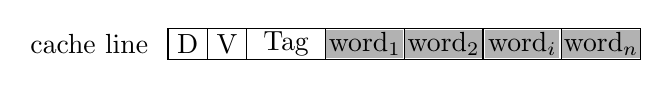
\begin{tikzpicture}
  \node[] (d) at (.25,0.2) {D};
  \node[] (v) at (.75,0.2) {V};
  \node[] (t) at (1.5,0.2) {Tag};
  \node[fill=gray!60] (w1) at (2.5,0.2) {word$_1$};
  \node[fill=gray!60] (w2) at (3.5,0.2) {word$_2$};
  \node[fill=gray!60] (wi) at (4.5,0.2) {word$_i$};
  \node[fill=gray!60] (wn) at (5.5,0.2) {word$_n$};
  \node[] (lb) at (-1,0.2) {cache line};
  \draw (0,0) rectangle (6,.4);
  \draw (.5,0) -- (.5,.4);
  \draw (1,0) -- (1,.4);
  \draw (2,0) -- (2,.4);
  \draw (3,0) -- (3,.4);
  \draw (4,0) -- (4,.4);
  \draw (5,0) -- (5,.4);
\end{tikzpicture}
\begin{itemize}
\item \textsf{D} (dirty) bit.  If $D=1$, data in cache modified and needs to be written back to main memory before eviction; if $D=0$, data clean and can be safely evicted without write-back
\item \textsf{V} (valid) bit.  If $V=1 \to$ data in cache line valid; if $V=0 \to$ cache line is empty or invalidated (should \emph{not} be read)
\item Tag bits contain the memory addr where the data is read from or written back to
\end{itemize}
\subsection*{False Sharing (severely affect parallel performance)}
\begin{itemize}
\item Condition where 2 processors write to different memory addresses but the addresses map to the same cache line
\item Suppose P$_1$ works on word$_j$ and P$_2$ works on word$_k$ (word$_j$ and word$_k$ are in the same cache line)
\item Each time $P_1$ or $P_2$ writes will (unnecessarily) invalidate the line and cause the other to wait for cache coherence; such ``ping-pong'' interactions cause high serialization overhead
\item use padding to alleviate the situations: P$_1$ pads its data so that the data with padding take up an entire cache line
\end{itemize}

% \pagebreak

\section*{Roofline Model (naive)}
\begin{minipage}{.6\linewidth}
  \flushleft
  \begin{itemize}
  \item max task-processing speed: \textcolor{red}{$P$ [flop/s]}
  \item bottleneck
    \begin{itemize}[label=-]
    \item execution of work: P$_{peak}$ [flop/s]
    \item data path: \textcolor{Green}{$I\cdot b_s$} [flop/byte $\cdot$ byte/s]
    \end{itemize}
  \end{itemize}
\[
\textcolor{red}{P} = \textsf{min}(\textcolor{Cyan}{P_{\text{peak}}}, \textcolor{Green}{I\cdot b_{s}})
\]
  \begin{itemize}
  \item High intensity: P limited by execution
  \item Low intensity: P limited by data transfer
  \item best use of resources (also max use of power): \textcolor{Tan}{Knee} at $P_{max} = I \cdot b_s$
  \item \textcolor{red}{roofline} is ``optimistic'' because it assumes data moves at \textcolor{red}{light speed}
  \end{itemize}
\end{minipage}
\begin{minipage}{.4\linewidth}
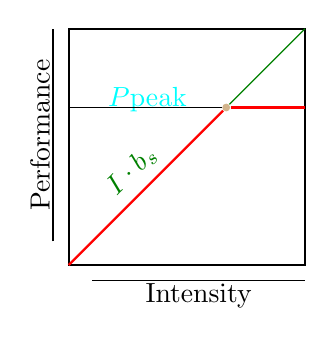
\begin{tikzpicture}
  % Knee
  \node[shape=circle,radius=1mm,fill=Tan]
  (knee) at (2,2) {};

  % Peaknode
  \node[color=Cyan] (peak) at (1,2.1) {$P\text{peak}$};

  % Ibsnode
  \node[color=Green,rotate=45] (ibs) at (.8,1.2)
  {$I\cdot b_s$};

  % rectangle coordinates
  \draw[thick] (0,0) rectangle (3,3);

  % y axis
  \draw (-.2, .3) edge[]
  node[above,sloped]{Performance} (-.2,3);

  % x axis
  \draw (.3, -.2) edge[]
  node[below]{Intensity} (3,-.2);

  % Peak
  \draw (0,2) -- (knee);
  \draw[color=red,thick] (knee) -- (3,2);

  % AI (I * Bs)
  \draw[color=red,thick] (0,0) -- (knee);
  \draw[color=Green] (knee) -- (3,3);

\end{tikzpicture}
\end{minipage}
\section*{CUDA}
\end{multicols*}
\end{document}
